%%%%%%%%%%%%%%%%%%%%%%%%%%%%%%%%%%%%%%%%%
% Jacobs Landscape Poster
% LaTeX Template
% Version 1.1 (14/06/14)
%
% Created by:
% Computational Physics and Biophysics Group, Jacobs University
% https://teamwork.jacobs-university.de:8443/confluence/display/CoPandBiG/LaTeX+Poster
% 
% Further modified by:
% Nathaniel Johnston (nathaniel@njohnston.ca)
%
% This template has been downloaded from:
% http://www.LaTeXTemplates.com
%
% License:
% CC BY-NC-SA 3.0 (http://creativecommons.org/licenses/by-nc-sa/3.0/)
%
%%%%%%%%%%%%%%%%%%%%%%%%%%%%%%%%%%%%%%%%%

%----------------------------------------------------------------------------------------
%	PACKAGES AND OTHER DOCUMENT CONFIGURATIONS
%----------------------------------------------------------------------------------------

\documentclass[final]{beamer}

\usepackage[scale=1.24]{beamerposter} % Use the beamerposter package for laying out the poster

\usetheme{confposter} % Use the confposter theme supplied with this template

\setbeamercolor{block title}{fg=ngreen,bg=white} % Colors of the block titles
\setbeamercolor{block body}{fg=black,bg=white} % Colors of the body of blocks
\setbeamercolor{block alerted title}{fg=white,bg=dblue!70} % Colors of the highlighted block titles
\setbeamercolor{block alerted body}{fg=black,bg=dblue!10} % Colors of the body of highlighted blocks
% Many more colors are available for use in beamerthemeconfposter.sty

%-----------------------------------------------------------
% Define the column widths and overall poster size
% To set effective sepwid, onecolwid and twocolwid values, first choose how many columns you want and how much separation you want between columns
% In this template, the separation width chosen is 0.024 of the paper width and a 4-column layout
% onecolwid should therefore be (1-(# of columns+1)*sepwid)/# of columns e.g. (1-(4+1)*0.024)/4 = 0.22
% Set twocolwid to be (2*onecolwid)+sepwid = 0.464
% Set threecolwid to be (3*onecolwid)+2*sepwid = 0.708

\newlength{\sepwid}
\newlength{\onecolwid}
\newlength{\twocolwid}
\newlength{\threecolwid}
\setlength{\paperwidth}{48in} % A0 width: 46.8in
\setlength{\paperheight}{36in} % A0 height: 33.1in
\setlength{\sepwid}{0.024\paperwidth} % Separation width (white space) between columns
\setlength{\onecolwid}{0.22\paperwidth} % Width of one column
\setlength{\twocolwid}{0.464\paperwidth} % Width of two columns
\setlength{\threecolwid}{0.708\paperwidth} % Width of three columns
\setlength{\topmargin}{-0.5in} % Reduce the top margin size
%-----------------------------------------------------------

\usepackage{graphicx}  % Required for including images
\usepackage{booktabs} % Top and bottom rules for tables
\usepackage{siunitx}
\usepackage[version=3]{mhchem}

\title{A Scalable Database for Sensor Observations} % Poster title

\author{Peter K. Kaiser\inst{1} \and John N. Doe\inst{2} \and Jutta Kaisaniemi\inst{3}} % Author(s)

\institute{\inst{1} Environmental Informatics Research Group, University of Zurich \and %
\inst{2} Biogeochemistry Research Group, Australian National University
\and %
\inst{3} College of Engineering and Computer Science, University of Eastern Finland} % Institution(s)

\begin{document}

\addtobeamertemplate{block end}{}{\vspace*{2ex}} % White space under blocks
\addtobeamertemplate{block alerted end}{}{\vspace*{2ex}} % White space under highlighted (alert) blocks

\setlength{\belowcaptionskip}{2ex} % White space under figures
\setlength\belowdisplayshortskip{2ex} % White space under equations

\begin{frame}[t] 

\begin{columns}[t] 
\begin{column}{\sepwid}\end{column}
\begin{column}{\onecolwid}

\begin{block}{Introduction}

NoSQL systems have been utilized to manage sensor observations, specifically. \cite{wang14hdsw} present a Hadoop-based system designed to manage sensor observations. 

Of particular interest here is CirrusRDF \cite{ladwig11cirrusrdf}. It has been widely adopted in the literature \cite{lefort12qb,phuoc11linked,mueller13restful}. The authors note that ``a complete `semantification' [...] of all data [...] seemed not feasible and promising to us, especially regarding the measurement data.'' 

As we discuss in more details, such systems generate large volumes of data, currently stored as files.
    
\end{block}

\begin{block}{Case Study}

We evaluate comparative database performance with data of a typical Sensor System for the direct measurement of \ce{CO2}, \ce{CH4}, and \ce{H2O} fluxes. Large data volumes for surface-atmosphere fluxes of energy and trace gases are managed by platforms such as SOCI Portal. The devices operate at \SI{10}{\hertz} sampling frequency and the data files include \SI{30}{\minute} of measurement. The total number of archive files is \num{1604500}. Each data file consists of a $\num{18000} \times 40$ matrix. Of this matrix, we concentrate on the three columns for measured \ce{CO2} [\si{\micro\mol\per\mol}], \ce{H2O} [\si{\milli\mol\per\mol}], and \ce{CH4} [\si{\micro\mol\per\mol}].

\end{block}

\setbeamercolor{block alerted title}{fg=black,bg=norange}
\setbeamercolor{block alerted body}{fg=black,bg=white}

\begin{alertblock}{Contact Information}

\begin{itemize}
\item Web: \href{http://www.university.edu/kaisaniemilab}{http://www.university.edu/kaisaniemilab}
\item Email: \href{mailto:j.kaisaniemi@example.org}{j.kaisaniemi@example.org}
\item Phone: +358 (000) 111 1111
\end{itemize}

\end{alertblock}

\begin{center}
  \begin{tabular}{ccc}
  
\includegraphics[width=0.4\linewidth]{marum.png} & \hfill &  
\includegraphics[width=0.4\linewidth]{unihb.png}
  \end{tabular}
\end{center}

\end{column}

\begin{column}{\sepwid}\end{column}
\begin{column}{\twocolwid}
\begin{block}{Results}

\begin{figure}
  \centering
  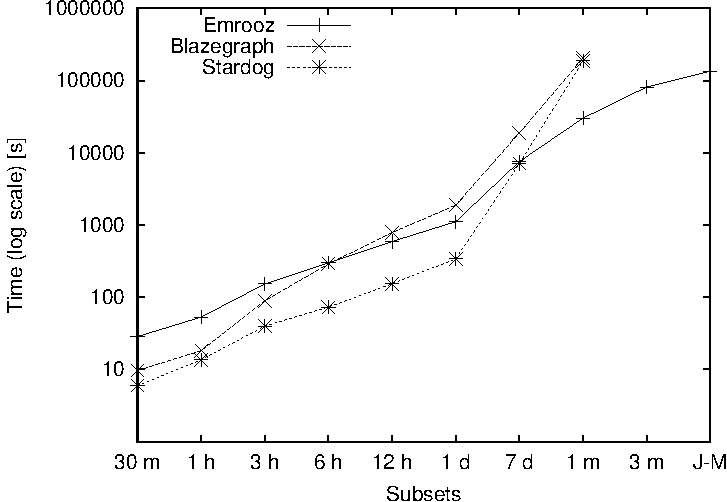
\includegraphics[scale=2]{load-performance-plot.pdf}
	\caption{A nice caption for the figure.}
	\label{fig:load-performance-plot}
\end{figure}

Figure \ref{fig:load-performance-plot} summarizes the \emph{load} performance for the 10 subsets compared to Stardog and Blazegraph. Figure \ref{fig:query-performance-plot} summarizes the \emph{query} performance for the 10 subsets compared to Stardog and Blazegraph. 

\begin{figure}
	\centering
	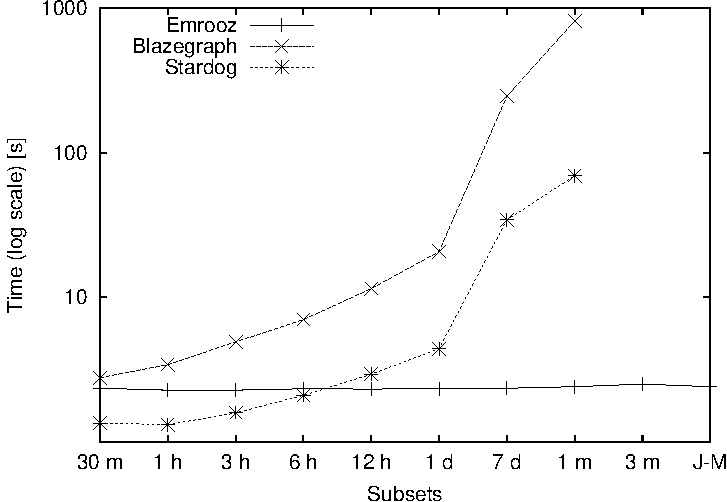
\includegraphics[scale=2]{query-performance-plot.pdf}
	\caption{Another nice caption for this second figure.}
	\label{fig:query-performance-plot}
\end{figure}

The database is capable of evaluating SPARQL queries with a basic graph pattern with \texttt{FILTER} and \texttt{ORDER BY}. The query performance is determined by the following complex mathematical expression

\begin{displaymath}
\lim_{x \to a} \frac{f(x) - f(a)}{x - a}
\end{displaymath}

\end{block}

\begin{block}{Conclusion}

We have presented a scalable database for sensor observations. That's it, folks! Thanks for reading.

\end{block}

\end{column} % End of the second column

\begin{column}{\sepwid}\end{column} % Empty spacer column

\begin{column}{\onecolwid} % The third column

\begin{block}{References}

\small{\bibliographystyle{unsrt}
\bibliography{bibliography}\vspace{0.75in}}

\end{block}

\setbeamercolor{block title}{fg=red,bg=white}

\begin{block}{Acknowledgements}

\small{\rmfamily{This research is funded by the Academy of Germany project ``ROTAR: High-quality Measurement Infrastructure'' (Grant number 5489654).}} \\

\end{block}

\end{column} % End of the third column
\end{columns} % End of all the columns in the poster
\end{frame} % End of the enclosing frame

\end{document}
